%%%%%%%%%%%%%%%%%%%%%%%%%%%%%%%%%%%%%%%%%
% Beamer Presentation
% LaTeX Template
% Version 1.0 (10/11/12)
%
% This template has been downloaded from:
% http://www.LaTeXTemplates.com
%
% License:
% CC BY-NC-SA 3.0 (http://creativecommons.org/licenses/by-nc-sa/3.0/)
%
%%%%%%%%%%%%%%%%%%%%%%%%%%%%%%%%%%%%%%%%%

%----------------------------------------------------------------------------------------
%	PACKAGES AND THEMES
%----------------------------------------------------------------------------------------

\documentclass{beamer}

\mode<presentation> {

% The Beamer class comes with a number of default slide themes
% which change the colors and layouts of slides. Below this is a list
% of all the themes, uncomment each in turn to see what they look like.

%\usetheme{default}
%\usetheme{AnnArbor}
%\usetheme{Antibes}
%\usetheme{Bergen}
%\usetheme{Berkeley}
%\usetheme{Berlin}
%\usetheme{Boadilla}
%\usetheme{CambridgeUS}
%\usetheme{Copenhagen}
%\usetheme{Darmstadt}
%\usetheme{Dresden}
%\usetheme{Frankfurt}
%\usetheme{Goettingen}
%\usetheme{Hannover}
%\usetheme{Ilmenau}
%\usetheme{JuanLesPins}
%\usetheme{Luebeck}
\usetheme{Madrid}
%\usetheme{Malmoe}
%\usetheme{Marburg}
%\usetheme{Montpellier}
%\usetheme{PaloAlto}
%\usetheme{Pittsburgh}
%\usetheme{Rochester}
%\usetheme{Singapore}
%\usetheme{Szeged}
%\usetheme{Warsaw}

% As well as themes, the Beamer class has a number of color themes
% for any slide theme. Uncomment each of these in turn to see how it
% changes the colors of your current slide theme.

%\usecolortheme{albatross}
%\usecolortheme{beaver}
%\usecolortheme{beetle}
%\usecolortheme{crane}
%\usecolortheme{dolphin}
%\usecolortheme{dove}
%\usecolortheme{fly}
%\usecolortheme{lily}
%\usecolortheme{orchid}
%\usecolortheme{rose}
%\usecolortheme{seagull}
%\usecolortheme{seahorse}
%\usecolortheme{whale}
%\usecolortheme{wolverine}

%\setbeamertemplate{footline} % To remove the footer line in all slides uncomment this line
%\setbeamertemplate{footline}[page number] % To replace the footer line in all slides with a simple slide count uncomment this line

%\setbeamertemplate{navigation symbols}{} % To remove the navigation symbols from the bottom of all slides uncomment this line
}

\usepackage{graphicx} % Allows including images
\usepackage{booktabs} % Allows the use of \toprule, \midrule and \bottomrule in tables

%----------------------------------------------------------------------------------------
%	TITLE PAGE
%----------------------------------------------------------------------------------------

\title[Anum - Akar Pers. Nonlinier]{Analisis Numerik\\Akar Persamaan Nonlinier} % The short title appears at the bottom of every slide, the full title is only on the title page

\author{Ahmad Rio Adriansyah} % Your name
\institute[STT-NF] % Your institution as it will appear on the bottom of every slide, may be shorthand to save space
{
STT Terpadu - Nurul Fikri \\ % Your institution for the title page
\medskip
\textit{ahmad.rio.adriansyah@gmail.com
\\arasy@nurulfikri.ac.id} % Your email address
}
\date{\today} % Date, can be changed to a custom date

\usepackage{graphicx}
\begin{document}

\begin{frame}
\titlepage % Print the title page as the first slide
\end{frame}

%----------------------------------------------------------------------------------------
%	PRESENTATION SLIDES
%----------------------------------------------------------------------------------------

%------------------------------------------------

\begin{frame}
\frametitle{Persamaan Non Linier}
Yang disebut persamaan non linier adalah :
\begin{enumerate}
\item polinom derajat $>$ 1
\item trigonometri
\item eksponensial
\item logaritma
\item dll
\end{enumerate}
\ \\\ \\Banyak persoalan di dunia nyata (matematika, sains, rekayasa) yang dimodelkan menjadi persamaan non linier
\end{frame}

%------------------------------------------------

\begin{frame}
\frametitle{Contoh}
Ketinggian gelombang berdiri (\textit{standing wave}) yang dipantulkan oleh dermaga diberikan oleh persamaan 
\begin{equation}
h = h_0 \biggl\{sin(\dfrac{2\pi x}{\lambda})cos(\omega t)+ e^{-x})\biggr\}
\nonumber
\end{equation}
dimana 
\begin{enumerate}
\item $h_0$ = ketinggian gelombang awal
\item $x$ = posisi longitudinal
\item $t$ = waktu longitudinal
\item $\lambda$ = panjang gelombang
\item $\omega$ = frekuensi angular
\end{enumerate}
Berapa jarak yang dibutuhkan agar tinggi gelombangnya menjadi separuhnya jika diketahui variabel $\lambda$, $\omega$, dan $t$ nya?
\end{frame}

%------------------------------------------------

\begin{frame}
\frametitle{Contoh}
Tingkat oksigen pada hilir sungai dari tempat pembuangan limbah dapat dituliskan sebagai fungsi
\begin{equation}
c = 10 - 15(e^{-0.1x}-e^{-0.5x})
\nonumber
\end{equation}
dimana $x$ adalah jarak tempat pengukuran pada hilir sungai dengan tempat pembuangan limbahnya.
\\\ \\Berapa jarak hilir sungai dari tempat pembuangan sampah jika hasil pengukurannya adalah 4? 
\end{frame}

%------------------------------------------------

\begin{frame}
\frametitle{Contoh}
Kecepatan sebuah roket dapat dihitung menggunakan 
\begin{equation}
v = u\ ln\biggl|\dfrac{m_0}{m_0-qt}\biggr| - gt
\nonumber
\end{equation}
dimana 
\begin{enumerate}
\item $u$ = kecepatan pada saat bahan bakar dikeluarkan
\item $m_0$ = massa awal roket, pada saat $t$=0
\item $q$ = laju pemakaian bahan bakar
\item $g$ = percepatan grafitasi
\end{enumerate}
\ \\\ \\kapan waktu roket tersebut mencapai kecepatan 1000 m/s?
\end{frame}

%------------------------------------------------

\begin{frame}
\frametitle{Deret Taylor}
Persamaan non linier bisa diubah jadi bentuk polinom dengan menggunakan deret Taylor
\end{frame}

%------------------------------------------------

\begin{frame}
\frametitle{Akar Persamaan}
Mencari akar dari fungsi $f(x)$ sama artinya dengan mencari nilai $x$ yang memenuhi persamaan $f(x)=0$.
\\\ \\Atau jika divisualisasikan dalam grafik, akar dari $f(x)$ adalah nilai $x$ pada saat grafik fungsi berpotongan dengan sumbu $x$
\begin{figure}[htp]
\centering
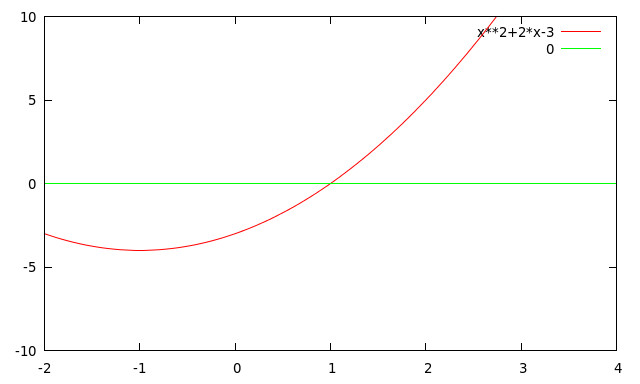
\includegraphics[scale=0.30]{Fungsi.jpg}
\end{figure}
\end{frame}

%------------------------------------------------

\begin{frame}
\frametitle{Akar Persamaan}
Contoh : 
\\Jika diberikan sebuah fungsi $f(x)= x^2+2x-3$ maka dengan mudah kita mengetahui bahwa akar-akarnya adalah $x_1 = -3$ dan $x_2 = 1$
\\\ \\Artinya, jika kita gambarkan grafik fungsi tersebut, maka akan berpotongan dengan sumbu $x$ di posisi $x = -3$ dan $x = 1$
\begin{figure}[htp]
\centering
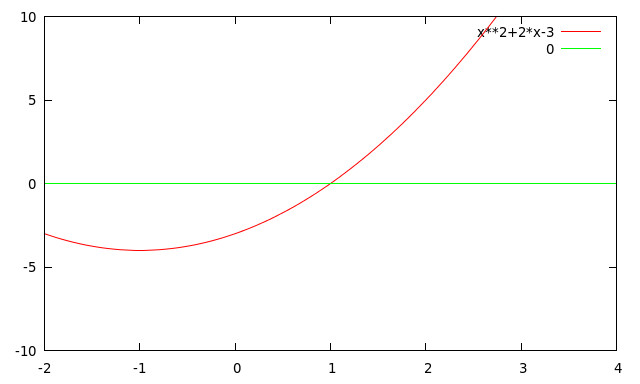
\includegraphics[scale=0.30]{Fungsi.jpg}
\end{figure}
\end{frame}

%------------------------------------------------

\begin{frame}
\frametitle{Metode Numerik}
Metode metode numerik yang digunakan untuk pencarian akar persamaan non linier ada sangat banyak ragamnya, tetapi secara umum dapat dikategorikan menjadi 2 kelompok besar :
\begin{enumerate}
\item Metode tertutup
\item Metode terbuka
\end{enumerate}
\end{frame}

%------------------------------------------------

\begin{frame}
\frametitle{Metode Tertutup}
Metode dalam kelompok ini mencari akar di dalam sebuah selang $[a,b]$ dengan dipastikan bahwa selang tersebut mengandung setidaknya sebuah akar. 
\\\ \\Dalam tiap iterasinya, lebar selang tersebut diperkecil secara sistematis dan semakin ujung-ujung selangnya konvergen menuju akar yang benar.
\\\ \\Metode yang termasuk kelompok ini diantaranya :
\begin{enumerate}
\item Metode bagidua (bisection / bolzano)
\item Metode posisi palsu (false position / regula falsi)
\end{enumerate}
\end{frame}

%------------------------------------------------

\begin{frame}
\frametitle{Metode Terbuka}
Metode dalam kelompok ini mencari akar tanpa perlu mengurung akar di dalam selang tertentu. Yang digunakan adalah tebakan awal $x_0$. 
\\\ \\Dalam tiap iterasinya, tebakan awal tersebut dipakai untuk menghitung hampiran akar yang baru secara sistematis. Hampiran akar ini bisa saja mendekati (konvergen) ke akar sejati, atau bahkan menjauhinya (divergen). Jadi metode ini tidak selalu menemukan akar sejati.
\\\ \\Metode yang termasuk kelompok ini diantaranya :
\begin{enumerate}
\item Metode titik tetap (fixed point)
\item Metode Newton-Raphson
\item Metode secant
\end{enumerate}
\end{frame}

%------------------------------------------------

\begin{frame}
\frametitle{Mencari Selang yang Mengandung Akar}
Bagaimana mencari selang yang mengandung akar dalam sebuah fungsi?
\\\ \\\ \\\ \\\ \\\ \\\ \\\ \\\ \\\ \\\ \\\ \\\
\end{frame}

%------------------------------------------------

\begin{frame}
\frametitle{Mencari Selang yang Mengandung Akar}
Bagaimana mencari selang yang mengandung akar dalam sebuah fungsi?
\\\ \\Ada 2 pendekatan yang bisa dilakukan :
\begin{enumerate}
\item Grafik \\Dibuat grafik fungsinya dalam bidang x-y, lalu dilihat perpotongan dengan sumbu x. Dari situ didapat perkiraan selang yang mengandung akarnya.
\item Kalkulasi \\Menentukan selang $[a,b]$, menghitung nilai fungsi di tepi selangnya $f(a)$ dan $f(b)$, lalu membandingkan tandanya. Jika tandanya berbeda, maka terdapat setidaknya satu akar di dalam selang tersebut.
\end{enumerate}
\end{frame}

%------------------------------------------------

\begin{frame}
\frametitle{Mencari Selang yang Mengandung Akar}
Teorema :
\\"Jika $f(x)$ kontinu dalam selang $[a,b]$ dan $f(a)f(b)<0$, maka paling sedikit terdapat satu buah akar persamaan $f(x)=0$ dalam selang $[a,b]$"
\begin{figure}[htp]
\centering
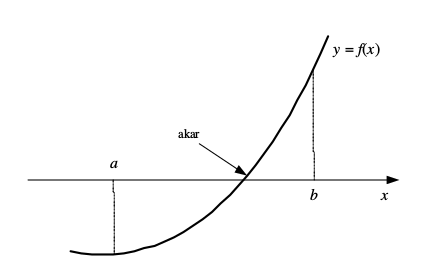
\includegraphics[scale=.50]{PosisiAkar.png}
\end{figure}
note : nilai fungsi dari ujung selang berbeda tanda adalah syarat cukup, tapi bukan syarat perlu
\end{frame}

%------------------------------------------------

\begin{frame}
\frametitle{Metode Bagi Dua (\textit{Bisection})}
Misalnya kita sudah menentukan selang tertutup $[a,b]$ dimana didalamnya sudah terdapat akar. \\\ \\Pada tiap iterasinya, metode ini membelah selang tersebut menjadi 2 subselang yang sama besar, yaitu $[a,c]$ dan $[c,b]$. \\\ \\Selang yang diambil untuk iterasi berikutnya adalah subselang yang memuat akar.
\end{frame}

%------------------------------------------------

\begin{frame}
\frametitle{Metode Bagi Dua}
\begin{figure}[htp]
\centering
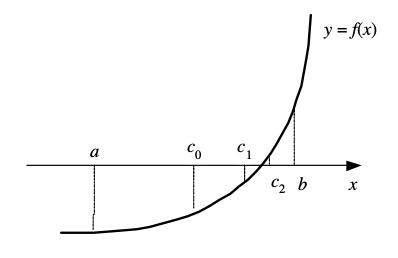
\includegraphics[scale=0.50]{AlurBagiDua.png}
\end{figure}
\end{frame}

%------------------------------------------------

\begin{frame}
\frametitle{Algoritma}
Input : $f(x)$, fungsi yang bersangkutan
\\\quad \qquad $a_0,b_0$, tebakan awal dimana $f(a_0)f(b_0)<0$
\\\quad \qquad $\epsilon_1,\epsilon_2$, toleransi galat
\\\ \\Output : hampiran akar dari $f(x)$ yang berada pada selang $[a_0,b_0]$
\\\ \\Untuk $k=0,1,2, ...$ sampai terpenuhi $|f(c_k)|<\epsilon_1$ atau $|b-a|<\epsilon_2$, lakukan :
\begin{enumerate}
\item Hitung $c_k = \dfrac{a_k+b_k}{2}$
\item Hitung $f(c_k)$
\item Jika $f(c_k)<\epsilon$, maka $c_k$ adalah akar. Jika tidak, kita periksa $f(a_k)f(c_k)$ atau $f(b_k)f(c_k)$. \\Jika $f(a_k)f(c_k)<0$, maka $a_{k+1}=a_k$ dan $b_{k+1}=c_k$
\\Jika sebaliknya, maka $a_{k+1}=c_k$ dan $b_{k+1}=b_k$
\end{enumerate} 
\end{frame}

%------------------------------------------------

\begin{frame}
\frametitle{Contoh}
Hitunglah akar dari fungsi $f(x)=x^2-4$, dengan \\tebakan awal $a_0=-1$ dan $b_0=7$. \\Kriteria pemberhentian dengan nilai fungsi lebih kecil dari $\epsilon_1 = 10^{-6}$ atau lebar selang lebih kecil dari $\epsilon_2 = 10^{-4}$.
\\\ \\\ \\\ \\\ \\\ \\\ \\
\begin{tabular}{llll}
\\
\
\end{tabular}
\\\ \\\
\\\ \\
\end{frame}

%------------------------------------------------

\begin{frame}
\frametitle{Penyelesaian}
Hitunglah akar dari fungsi $f(x)=x^2-4$, dengan \\tebakan awal $a_0=-1$ dan $b_0=7$. \\Kriteria pemberhentian dengan nilai fungsi lebih kecil dari $\epsilon_1 = 10^{-6}$ atau lebar selang lebih kecil dari $\epsilon_2 = 10^{-4}$.
\\\ \\Secara analitik, kita bisa menjawab berapa akar fungsi tersebut, tapi di sini akan ditunjukkan cara numeriknya. Pertama-tama, kita periksa terlebih dahulu apakah tebakan awal yang kita gunakan sudah mengapit salah satu akar atau belum.
\\\ \\
\begin{tabular}{llll}
$f(a_0)$ & $= f(-1)$ & $= (-1)^2-4$ & $= -3$\\
$f(b_0)$ & $= f(7)$ & $= (7)^2-4$ & $= 45$
\end{tabular}
\\\ \\Hasil kali $f(a_0)$ dan $f(b_0)$ = $(-3)(45) =-135$ , lebih kecil dari nol.
\\Dari teorema, berarti kita bisa pastikan bahwa setidaknya ada satu akar berada pada selang $[-1,7]$
\end{frame}

%------------------------------------------------

\begin{frame}
\frametitle{Penyelesaian}
\begin{tabular}{|c|c|c|c|c|c|c|}
\hline
	$i$ & $a_i$ & $f(a_i)$ & $b_i$ & $f(b_i)$ & $c_i$ & $f(c_i)$\\
\hline
	0 & -1 & -3 & 7 & 45 & $\dfrac{(-1)+7}{2}=\dfrac{6}{2}=3$ & 5\\
\hline
	1 &  &  &  &  &  & \\
\hline
	2 &  &  &  &  &  & \\
\hline
	3 &  &  &  &  &  & \\
\hline
	4 &  &  &  &  &  & \\
\hline
\end{tabular}
\\\ \\$c_0$ (titik tengah pertama) didapat dari hasil tengah-tengah nilai $a_0$ dan $b_0$
\\bisa dihitung dengan rumus 
\begin{equation}
c_i= \dfrac{a_i+b_i}{2}
\nonumber
\end{equation}
tapi bisa terjadi overflow karena adanya penjumlahan $a$ dan $b$ (jika angkanya besar). Alternatifnya, nilai $c_0$ dan seterusnya dapat dihitung dengan rumus 
\begin{equation}
c_i= a_i + \dfrac{b_i-a_i}{2}
\nonumber
\end{equation}
\end{frame}

%------------------------------------------------

\begin{frame}
\frametitle{Penyelesaian}
\begin{tabular}{|c|c|c|c|c|c|c|}
\hline
	$i$ & $a_i$ & $f(a_i)$ & $b_i$ & $f(b_i)$ & $c_i$ & $f(c_i)$\\
\hline
	0 & -1 & -3 & 7 & 45 & $\qquad\quad\ $ 3 $\qquad\quad\ $  & 5\\
\hline
	1 &  &  &  &  &  & \\
\hline
	2 &  &  &  &  &  & \\
\hline
	3 &  &  &  &  &  & \\
\hline
	4 &  &  &  &  &  & \\
\hline
\end{tabular}
\\\ \\Kita lihat hasil kali $f(a)f(c) = (-3)(5) = -15$, ternyata lebih kecil dari nol. \\\ \\Jika $f(a)f(c)<0$, berarti akarnya berada diantara selang $[a,c]$. Kita bisa ganti nilai $b$ pada iterasi selanjutnya dengan nilai $c$ untuk mendapatkan selang yang lebih kecil. 
\end{frame}

%------------------------------------------------

\begin{frame}
\frametitle{Penyelesaian}
\begin{tabular}{|c|c|c|c|c|c|c|}
\hline
	$i$ & $a_i$ & $f(a_i)$ & $b_i$ & $f(b_i)$ & $c_i$ & $f(c_i)$\\
\hline
	0 & -1 & -3 & 7 & 45 & $\qquad\quad\ $ 3 $\qquad\quad\ $  & 5\\
\hline
	1 & -1 & -3 & \textbf{3} & \textbf{5} &  & \\
\hline
	2 &  &  &  &  &  & \\
\hline
	3 &  &  &  &  &  & \\
\hline
	4 &  &  &  &  &  & \\
\hline
\end{tabular}
\\\ \\Kita bandingkan hasil kali $f(a)f(c) = (-3)(5) = -15$, ternyata lebih kecil dari nol. \\\ \\Jika $f(a)f(c)<0$, berarti akarnya berada diantara selang $[a,c]$. Kita bisa ganti nilai $b$ pada iterasi selanjutnya dengan nilai $c$ untuk mendapatkan selang yang lebih kecil. 
\end{frame}

%------------------------------------------------

\begin{frame}
\frametitle{Penyelesaian}
\begin{tabular}{|c|c|c|c|c|c|c|}
\hline
	$i$ & $a_i$ & $f(a_i)$ & $b_i$ & $f(b_i)$ & $c_i$ & $f(c_i)$\\
\hline
	0 & -1 & -3 & 7 & 45 & $\qquad\quad\ $ 3 $\qquad\quad\ $  & 5\\
\hline
	1 & -1 & -3 & \textbf{3} & \textbf{5} &  $-1+\dfrac{3-(-1)}{2}=1$ & -3\\
\hline
	2 &  &  &  &  &  & \\
\hline
	3 &  &  &  &  &  & \\
\hline
	4 &  &  &  &  &  & \\
\hline
\end{tabular}
\\\ \\Dihitung kembali nilai $c_1$ dan $f(c_1)$
\\\ \\$f(x) = x^2 - 4$
\\$f(1) = 1^2 - 4 = -3$
\\\ \\Kali ini hasil kali $f(c)f(b)<0$, berarti di iterasi selanjutnya selang yang digunakan adalah selang $[c,b]$
\end{frame}

%------------------------------------------------
\begin{frame}
\frametitle{Penyelesaian}
\begin{tabular}{|c|c|c|c|c|c|c|}
\hline
	$i$ & $a_i$ & $f(a_i)$ & $b_i$ & $f(b_i)$ & $c_i$ & $f(c_i)$\\
\hline
	0 & -1 & -3 & 7 & 45 & $\qquad\quad\ $ 3 $\qquad\quad\ $  & 5\\
\hline
	1 & -1 & -3 & \textbf{3} & \textbf{5} &  1 & -3\\
\hline
	2 & \textbf{1} & \textbf{-3} & 3 & 5 &  $\dfrac{1+3}{2}=\dfrac{4}{2}=2$ & 0\\
\hline
	3 &  &  &  &  &  & \\
\hline
	4 &  &  &  &  &  & \\
\hline
\end{tabular}
\\\ \\Pada langkah ini, ternyata $f(c) = 0 < \epsilon$, dengan kata lain kita sudah menemukan akar yang kita cari, yaitu $c = 2$ 
\\\ \\Salah satu akar dari persamaan $f(x) = x^2-4$ adalah $x=2$

\end{frame}

%------------------------------------------------

\begin{frame}
\frametitle{Algoritma Metode Bagi Dua (Revisi)}
Input : $f(x)$, fungsi yang bersangkutan
\\\quad \qquad $a_0,b_0$, tebakan awal dimana $f(a_0)f(b_0)<0$
\\\quad \qquad $\epsilon_1, \epsilon_2$, toleransi galat
\\\ \\Output : hampiran akar dari $f(x)$ yang berada pada selang $[a_0,b_0]$
\\\ \\Untuk $k=0,1,2, ...$ sampai terpenuhi $|f(c_k)|<\epsilon_1$ atau $|b-a|<\epsilon_2$, lakukan :
\begin{enumerate}
\item Hitung $c_k = a_k + \dfrac{b_k-a_k}{2}$
\item Hitung $f(c_k)$
\item Jika $f(c_k)<\epsilon$, maka $c_k$ adalah akar. Jika tidak, kita periksa $f(a_k)f(c_k)$ atau $f(b_k)f(c_k)$. \\\qquad Jika $f(a_k)f(c_k)<0$, maka $a_{k+1}=a_k$ dan $b_{k+1}=c_k$
\\\qquad Jika sebaliknya, maka $a_{k+1}=c_k$ dan $b_{k+1}=b_k$
\end{enumerate} 
\end{frame}

%------------------------------------------------

\begin{frame}
\frametitle{Metode Bagi Dua}
Salah satu kriteria pemberhentian bagi metode bagi dua adalah lebar selang yang dicapai. Jika lebar selangnya lebih kecil dari $\epsilon_2$, maka iterasi diberhentikan.
\\\ \\
Iterasi maksimal yang dibutuhkan oleh metode bagi dua untuk mencapai hampiran akar yang errornya kurang dari $\epsilon_2$ pada selang $[a,b]$ adalah
\begin{equation}
R > \dfrac{ln(|b-a|)-ln(\epsilon_2)}{ln(2)}
\nonumber
\end{equation}
atau 
\begin{equation}
R >\ ^2log\biggl(\dfrac{|b-a|}{\epsilon_2}\biggr)
\nonumber
\end{equation}
\end{frame}

%------------------------------------------------

\begin{frame}
\frametitle{Latihan}
Cari nilai salah satu akar dari fungsi $f(x) = 16x^3 -22x +9$ menggunakan metode bagi dua dengan selang tebakan awal :
\begin{enumerate}
\item $[-2,-1]$
\item $[0.2,0.7]$
\item $[0.7,1]$
\end{enumerate}
\ \\\ \\
hingga galatnya lebih kecil dari $10^{-4}$ atau maksimal 8 iterasi 
\\\ \\note : gunakan perhitungan 4 angka di belakang koma
\end{frame}

%------------------------------------------------

\begin{frame}
\frametitle{Tugas}
Opsi 1 :\\\ \\
Buat implementasi metode bagi dua dalam python. \\\ \\Input fungsi dan batas galat boleh di\textit{hardcode}kan, tapi input selang awal dimasukkan oleh user. Input selang diperiksa terlebih dahulu apakah di dalamnya mengandung akar atau tidak.
\end{frame}

%------------------------------------------------

\begin{frame}
\frametitle{Metode Posisi Palsu (\textit{Regula Falsi})}
Metode bagi dua selalu menemukan akar, tetapi kecepatan konvergensinya lambat. Kecepatan konvergensi bisa ditingkatkan jika nilai $f(a)$ dan $f(b)$ diperhitungkan juga. Jika $|f(a)|<|f(b)|$, maka nilai akar logikanya lebih dekat ke $a$, daripada $b$.\\\ \\Metode posisi palsu memanfaatkan hal tersebut. Pada tiap iterasinya, ditarik garis antara nilai $f(a)$ dan $f(b)$. Titik perpotongan garis tersebut dengan sumbu $x$ digunakan sebagai nilai penentu selang yang baru.
\end{frame}

%------------------------------------------------

\begin{frame}
\frametitle{Metode Posisi Palsu}
\begin{figure}[htp]
\centering
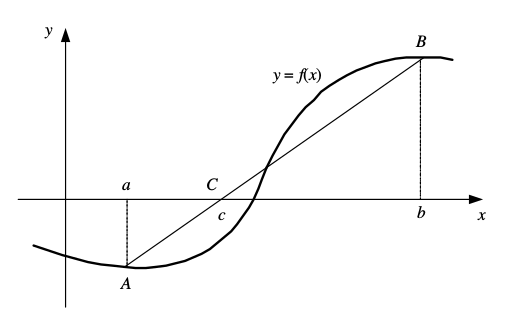
\includegraphics[scale=0.50]{AlurPosisiPalsu.png}
\end{figure}
\end{frame}

%------------------------------------------------

\begin{frame}
\frametitle{Metode Posisi Palsu}
Nilai c dapat dicari dengan menggunakan persamaan garis lurus yang melalui dua buah titik
\begin{equation}
c = a - \biggl(\dfrac{f(a)}{f(b)-f(a)}\biggr)(b-a)
\end{equation}
atau
\begin{equation}
c = b - \biggl(\dfrac{f(b)}{f(b)-f(a)}\biggr)(b-a)
\end{equation}
\ \\\ \\Pada contoh algoritma ini, kita gunakan persamaan (2)
\end{frame}

%------------------------------------------------

\begin{frame}
\frametitle{Algoritma}
Input : $f(x)$, fungsi yang bersangkutan
\\\quad \qquad $a_0,b_0$, tebakan awal dimana $f(a_0)f(b_0)<0$
\\\quad \qquad $\epsilon_1,\epsilon_2$, toleransi galat
\\\ \\Output : hampiran akar dari $f(x)$ yang berada pada selang $[a_0,b_0]$
\\\ \\Untuk $k=0,1,2, ...$ sampai terpenuhi $|f(c_k)|<\epsilon_1$ atau $|b-a|<\epsilon_2$, lakukan :
\begin{enumerate}
\item Hitung $c_k = b_k - \biggl(\dfrac{f(b_k)}{f(b_k)-f(a_k)}\biggr)(b_k-a_k)$
\item Hitung $f(c_k)$
\item Jika $f(c_k)<\epsilon$, maka $c_k$ adalah akar. Jika tidak, kita periksa $f(a_k)f(c_k)$ atau $f(b_k)f(c_k)$. \\Jika $f(a_k)f(c_k)<0$, maka $a_{k+1}=a_k$ dan $b_{k+1}=c_k$
\\Jika sebaliknya, maka $a_{k+1}=c_k$ dan $b_{k+1}=b_k$
\end{enumerate} 
\end{frame}

%------------------------------------------------

\begin{frame}
\frametitle{Contoh}
Sama seperti yang kita kerjakan pada metode bagi dua. Hitunglah akar dari fungsi $f(x)=x^2-4$, dengan \\tebakan awal $a_0=-1$ dan $b_0=7$ menggunakan metode posisi palsu. \\\ \\Kriteria pemberhentiannya adalah jika nilai fungsi lebih kecil dari $\epsilon_1 = 10^{-6}$ atau lebar selang lebih kecil dari $\epsilon_2 = 10^{-4}$.
\\\ \\Dari teorema sebelumnya, kita sudah tahu bahwa setidaknya ada satu akar berada pada selang $[-1,7]$
\\\ \\Secara umum, metode posisi palsu mirip seperti metode bagi dua, selain cara perhitungan c nya. 
\\\ \\
\end{frame}

%------------------------------------------------

\begin{frame}
\frametitle{Penyelesaian}
\begin{tabular}{|c|c|c|c|c|l|c|}
\hline
	$i$ & $a_i$ & $f(a_i)$ & $b_i$ & $f(b_i)$ & $c_i$ & $f(c_i)$\\
\hline
	0 & -1 & -3 & 7 & 45 & $7 - \biggl(\dfrac{45}{45-(-3)}\biggr)(7-(-1))$ & -3.75\\
	  &  &  &  &  & $=7 - (0.9375)(8)$  & \\
	  &  &  &  &  & $=7 - 7.5$  & \\
	  &  &  &  &  & $=-0.5$  & \\
\hline
	1 &  &  &  &  &  & \\
\hline
	2 &  &  &  &  &  & \\
\hline
\end{tabular}
\\\ \\$c_0$ (titik hampiran pertama) didapat dari hasil perpotongan garis antara sumbu $x$ dengan garis yang menghubungkan dua titik $(a_0,f(a_0))$ dan $(b_0,f(b_0))$
\\bisa dihitung dengan rumus 
\begin{equation}
c_0 = b_0 - \biggl(\dfrac{f(b_0)}{f(b_0)-f(a_0)}\biggr)(b_0-a_0)\nonumber
\end{equation}
\end{frame}

%------------------------------------------------

\begin{frame}
\frametitle{Latihan}
Cari nilai salah satu akar dari fungsi $f(x) = 16x^3 -22x +9$ menggunakan metode posisi palsu dengan selang tebakan awal :
\begin{enumerate}
\item $[-2,-1]$
\item $[0.2,0.7]$
\item $[0.7,1]$
\end{enumerate}
\ \\\ \\
hingga galatnya lebih kecil dari $10^{-4}$ atau maksimal 8 iterasi 
\\\ \\note : gunakan perhitungan 4 angka di belakang koma
\end{frame}

%------------------------------------------------

\begin{frame}
\frametitle{Tugas}
Opsi 2 :\\\ \\
Buat implementasi metode posisi palsu dalam python. \\\ \\Input fungsi dan batas galat boleh di\textit{hardcode}kan, tapi input selang awal dimasukkan oleh user. Input selang diperiksa terlebih dahulu apakah di dalamnya mengandung akar atau tidak.
\end{frame}

%------------------------------------------------

\begin{frame}
\frametitle{Metode Terbuka}
Metode dalam kelompok ini mencari akar tanpa perlu mengurung akar di dalam selang tertentu. Yang digunakan adalah tebakan awal $x_0$. 
\\\ \\Dalam tiap iterasinya, tebakan awal tersebut dipakai untuk menghitung hampiran akar yang baru secara sistematis. Hampiran akar ini bisa saja mendekati (konvergen) ke akar sejati, atau bahkan menjauhinya (divergen). Jadi metode ini tidak selalu menemukan akar sejati.
\\\ \\Metode yang termasuk kelompok ini diantaranya :
\begin{enumerate}
\item Metode titik tetap (fixed point)
\item Metode Newton-Raphson
\item Metode secant
\end{enumerate}

\end{frame}

%------------------------------------------------

\begin{frame}
\frametitle{Metode Iterasi Titik Tetap}
Metode ini kadang disebut sebagai metode iterasi sederhana atau metode langsung. Kesederhanaannya karena prosedur iterasinya yang mudah dibentuk sebagai berikut :
\begin{enumerate}
\item Susun $f(x) = 0$ menjadi $x = g(x)$
\item Bentuk persamaan tersebut menjadi prosedur iteratif
\begin{equation}
x_{r+1} = g(x_r)
\nonumber
\end{equation}
\item Tentukan sebuah nilai awal $x_0$
\item Hitung $x_1,x_2,$ dst sehingga konvergen
\begin{equation}
f(x_s) = 0 \text{ dan } x_{s} = g(x_s)
\nonumber
\end{equation}
\end{enumerate}
\end{frame}

%------------------------------------------------

\begin{frame}
\frametitle{Algoritma}
Input : $g(x)$, fungsi hasil modifikasi dari $f(x)=0$
\\\quad \qquad $x$, tebakan awal
\\\quad \qquad $\epsilon$, toleransi galat
\\\ \\Output : $x$, hampiran akar dari $f(x)$
\\\ \\Untuk $k=0,1,2, ...$ sampai terpenuhi $|x-x\_sebelumnya|<\epsilon$, lakukan :
\begin{enumerate}
\item x\_sebelumnya = $x$
\item Hitung $x = g(x\_sebelumnya)$
\item Jika $|x-x\_sebelumnya|<\epsilon$, maka $x$ adalah akar dari $f(x)$
\end{enumerate} 
\end{frame}

%------------------------------------------------

\begin{frame}
\frametitle{Contoh}
Hitunglah akar dari fungsi $f(x)=x^2+2x-3$, dengan tebakan awal $x_0=2$. \\Kriteria pemberhentian ketika errornya sudah lebih kecil dari $\epsilon = 10^{-6}$ 
\\\ \\\ 
\\\ \\\ 
\begin{equation}
\begin{split}
\ 
\\\ 
\\\
\end{split}
\nonumber
\end{equation}
\end{frame}

%------------------------------------------------

\begin{frame}
\frametitle{Contoh}
Hitunglah akar dari fungsi $f(x)=x^2+2x-3$, dengan tebakan awal $x_0=2$. \\Kriteria pemberhentian ketika errornya sudah lebih kecil dari $\epsilon = 10^{-6}$ 
\\\ \\Langkah pertama, ubah persamaan fungsi $f(x)=0$ menjadi $x=g(x)$
\\\ \\$f(x) = x^2+2x-3 = 0$ dapat diubah bentuknya menjadi 
\begin{equation}
\begin{split}
x^2+2x-3 &= 0
\\2x &= 3-x^2
\\x & = \dfrac{3-x^2}{2}
\end{split}
\nonumber
\end{equation}
\end{frame}

%------------------------------------------------

\begin{frame}
\frametitle{Penyelesaian}
\begin{equation}
g(x) = \dfrac{3-x^2}{2}
\nonumber
\end{equation}
tebakan awal $x_0=2$
\\\begin{center}
\begin{tabular}{|c|c|c|c|}
\hline
	$i$ & $x_i$ & $x_{i+1} = g(x_i)$ & galat \\
\hline
	0 & 2 & $\dfrac{3 - (2)^2}{2} = -0.5$ & -\\
\hline
	1 &  &  & \\
\hline
	2 &  &  & \\
\hline
	3 &  &  & \\
\hline
\end{tabular}
\end{center}
\end{frame}

%------------------------------------------------

\begin{frame}
\frametitle{Penyelesaian}
\begin{equation}
g(x) = \dfrac{3-x^2}{2}
\nonumber
\end{equation}
tebakan awal $x_0=2$
\\\begin{center}
\begin{tabular}{|c|c|c|c|}
\hline
	$i$ & $x_i$ & $x_{i+1} = g(x_i)$ & galat \\
\hline
	0 & 2 & $-0.5$ & -\\
\hline
	1 & $-0.5$ & $\dfrac{3 - (-0.5)^2}{2} = 1.375$ & $|1.375 - (-0.5)| = 1.875$ \\
\hline
	2 &  &  & \\
\hline
	3 &  &  & \\
\hline
\end{tabular}
\end{center}
\end{frame}

%------------------------------------------------

\begin{frame}
\frametitle{Penyelesaian}
\begin{equation}
g(x) = \dfrac{3-x^2}{2}
\nonumber
\end{equation}
tebakan awal $x_0=2$
\\\begin{center}
\begin{tabular}{|c|c|c|c|}
\hline
	$i$ & $x_i$ & $x_{i+1} = g(x_i)$ & galat \\
\hline
	0 & $2$ & $-0.5$ & -\\
\hline
	1 & $-0.5$ & $1.375$ & $1.875$ \\
\hline
	2 & $1.375$ & $\dfrac{3 - (1.375)^2}{2} = 0.5547$ & $| 0.5547 - 1.375| = 0.8203$ \\
\hline
	3 &  &  & \\
\hline
\end{tabular}
\end{center}
dst...
\end{frame}

%------------------------------------------------

\begin{frame}
\frametitle{Metode Titik Tetap}
Metode ini tidak selalu menghasilkan iterasi yang konvergen ke akar, bisa pula divergen tergantung pada :
\begin{enumerate}
\item fungsi $g(x)$ yang dibentuk
\item titik tebakan awal
\end{enumerate}
\ \\\ \\Dari fungsi $f(x)$ yang sama dapat dibentuk beberapa macam $g(x)$. Contohnya fungsi $f(x) = x^2-2x-3$ dapat dibentuk jadi
\begin{enumerate}
\item $g(x) = \dfrac{x^2-3}{2}$
\item \qquad - \qquad - \qquad - \qquad $g(x) = \sqrt{2x+3}$, atau
\item $g(x) = \dfrac{3}{x-2}$
\end{enumerate}
\end{frame}

%------------------------------------------------

\begin{frame}
\frametitle{Metode Titik Tetap}
Jika diberikan nilai awal yang sama, yaitu $x_0 = 4$, perilaku ketiga fungsi tersebut berbeda dalam mencari akar persamaannya.
\\\ \\$g(x) = \dfrac{x^2-3}{2}$
\begin{figure}[htp]
\centering
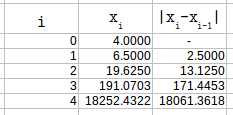
\includegraphics[scale=0.80]{TTver1.png}
\end{figure}
Hasilnya \textbf{divergen}, semakin membesar (ke arah $\infty$) atau semakin mengecil (ke arah $-\infty$)
\end{frame}

%------------------------------------------------

\begin{frame}
\frametitle{Metode Titik Tetap}
$g(x) = \sqrt{2x+3}$
\begin{figure}[htp]
\centering
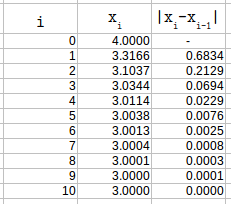
\includegraphics[scale=0.70]{TTver2.png}
\end{figure}
Hasilnya \textbf{konvergen monoton}, ke arah satu titik tertentu, dalam hal ini $x=3$
\end{frame}

%------------------------------------------------

\begin{frame}
\frametitle{Metode Titik Tetap}
$g(x) = \dfrac{3}{x-2}$
\begin{figure}[htp]
\centering
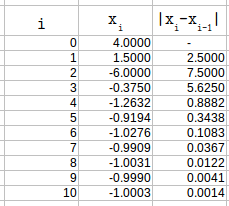
\includegraphics[scale=0.70]{TTver3.png}
\end{figure}
Hasilnya \textbf{konvergen berosilasi}, ke arah satu titik tertentu, dalam hal ini $x=-1$
\end{frame}

%------------------------------------------------

\begin{frame}
\frametitle{Metode Titik Tetap}
Demikian pula jika fungsi yang digunakan sama, tetapi nilai tebakan awal yang digunakan berbeda.
\\\ \\Misalnya fungsi $f(x) = x^3+6x-3$ dengan fungsi iterasi yang digunakan $x_{r+1}= \dfrac{3-x_{r}^3}{6}$ dengan tebakan awal $x_0= \{0.5,\ 1.5,\ 2.2,\ 2.7\}$
\begin{figure}[htp]
\centering
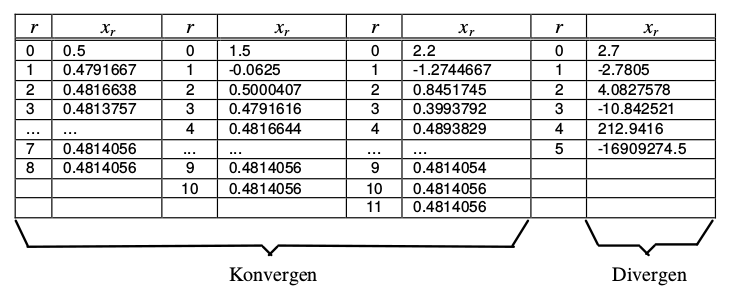
\includegraphics[scale=0.47]{TitikTetapmultix0.png}
\end{figure}\end{frame}

%------------------------------------------------

\begin{frame}
\frametitle{Tugas}
Opsi 3 :\\\ \\
Buat implementasi metode titik tetap dalam python. \\\ \\Input fungsi dan batas galat boleh di\textit{hardcode}kan, tapi input tebakan awal dimasukkan oleh user. 
\end{frame}

%------------------------------------------------

\begin{frame}
\frametitle{Metode Newton-Raphson}
Metode ini adalah metode yang paling terkenal sebagai metode pencarian akar, dan banyak digunakan dalam bidang sains dan rekayasa. Metode ini disukai karena konvergensinya paling cepat diantara metode lainnya.
\\\ \\Ada dua pendekatan dalam penurunan metode Newton-Raphson
\begin{enumerate}
\item Secara geometri
\item Memanfaatkan deret Taylor
\begin{equation}
f(x_s) = 0 \text{ dan } x_{s} = g(x_s)
\nonumber
\end{equation}
\end{enumerate}
\end{frame}

%------------------------------------------------

\begin{frame}
\frametitle{Metode Newton-Raphson (Geometri)}
\begin{figure}[htp]
\centering
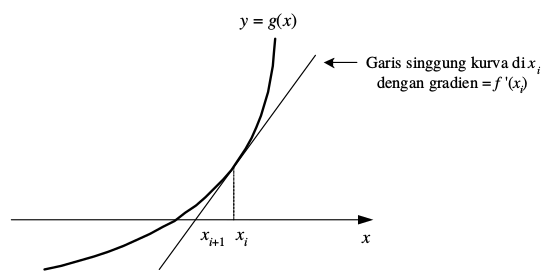
\includegraphics[scale=0.60]{NewtonRaphsonGeometri.png}
\end{figure}
\end{frame}

%------------------------------------------------

\begin{frame}
\frametitle{Metode Newton-Raphson (Geometri)}
Gradien dari garis singgung $f(x)$ di titik $x_r$ adalah
\begin{equation}
\begin{split}
m = f'(x_r) &= \dfrac{\Delta y}{\Delta x} = \dfrac{f(x_r)-0}{x_r - x_{r+1}}
\\f'(x_r) &= \dfrac{f(x_r)}{x_r - x_{r+1}}
\end{split}
\nonumber
\end{equation}
dengan kata lain, 
\begin{equation}
x_{r+1}  =x_r - \dfrac{f(x_r)}{f'(x_r)}
\nonumber
\end{equation}
\end{frame}

%------------------------------------------------

\begin{frame}
\frametitle{Metode Newton-Raphson (Deret Taylor)}
Uraikan $f(x_{r+1})$ di sekitar $x_r$ menggunakan deret Taylor didapatkan
\begin{equation}
\begin{split}
f(x_{r+1}) &= f(x_r)+ (x_{r+1}-x_r)f'(x_r)+\dfrac{(x_{r+1}-x_r)^2}{2!}f''(x_r) + \dots\\
f(x_{r+1}) &\approx f(x_r)+ (x_{r+1}-x_r)f'(x_r)
\end{split}
\nonumber
\end{equation}
Karena ini adalah permasalahan mencari akar, maka $f(x_{r+1})=0$, dengan kata lain, 
\begin{equation}
x_{r+1}  =x_r - \dfrac{f(x_r)}{f'(x_r)}
\nonumber
\end{equation}
\end{frame}

%------------------------------------------------

\begin{frame}
\frametitle{Metode Newton-Raphson}
Cara metode Newton-Raphson mendekati nilai sejati sama seperti cara metode titik tetap. Nilai hampiran $x_i$ diperbaiki terus menerus dalam tiap iterasinya. Yang membedakan adalah cara pengambilan nilai $x$ yang baru, yaitu menggunakan formula
\begin{equation}
x_{r+1}  =x_r - \dfrac{f(x_r)}{f'(x_r)}
\nonumber
\end{equation}
\end{frame}

%------------------------------------------------

\begin{frame}
\frametitle{Tugas}
Opsi 4 :\\\ \\
Buat implementasi metode Newton-Raphson dalam python. \\\ \\Input fungsi, turunan fungsi, dan batas galat boleh di\textit{hardcode}kan, tapi input tebakan awal dimasukkan oleh user. 
\end{frame}

%------------------------------------------------

\end{document} 